% Created by tikzDevice version 0.10.1 on 2016-08-01 16:03:33
% !TEX encoding = UTF-8 Unicode
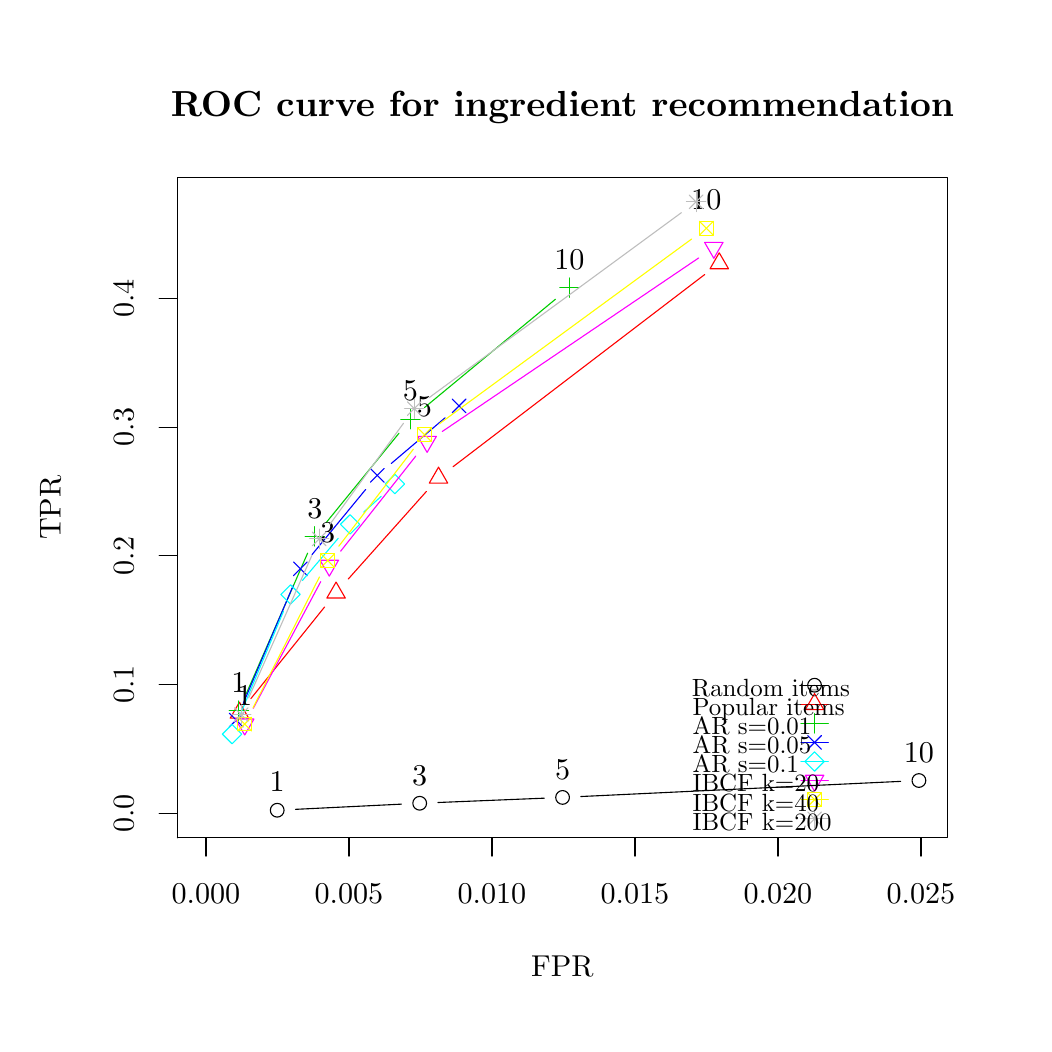
\begin{tikzpicture}[x=1pt,y=1pt]
\definecolor{fillColor}{RGB}{255,255,255}
\path[use as bounding box,fill=fillColor,fill opacity=0.00] (0,0) rectangle (360.07,360.07);
\begin{scope}
\path[clip] (  0.00,  0.00) rectangle (360.07,360.07);
\definecolor{drawColor}{RGB}{0,0,0}

\path[draw=drawColor,line width= 0.4pt,line join=round,line cap=round] ( 64.42, 67.32) -- (322.78, 67.32);

\path[draw=drawColor,line width= 0.4pt,line join=round,line cap=round] ( 64.42, 67.32) -- ( 64.42, 60.72);

\path[draw=drawColor,line width= 0.4pt,line join=round,line cap=round] (116.10, 67.32) -- (116.10, 60.72);

\path[draw=drawColor,line width= 0.4pt,line join=round,line cap=round] (167.77, 67.32) -- (167.77, 60.72);

\path[draw=drawColor,line width= 0.4pt,line join=round,line cap=round] (219.44, 67.32) -- (219.44, 60.72);

\path[draw=drawColor,line width= 0.4pt,line join=round,line cap=round] (271.11, 67.32) -- (271.11, 60.72);

\path[draw=drawColor,line width= 0.4pt,line join=round,line cap=round] (322.78, 67.32) -- (322.78, 60.72);

\node[text=drawColor,anchor=base,inner sep=0pt, outer sep=0pt, scale=  1.09] at ( 64.42, 43.56) {0.000};

\node[text=drawColor,anchor=base,inner sep=0pt, outer sep=0pt, scale=  1.09] at (116.10, 43.56) {0.005};

\node[text=drawColor,anchor=base,inner sep=0pt, outer sep=0pt, scale=  1.09] at (167.77, 43.56) {0.010};

\node[text=drawColor,anchor=base,inner sep=0pt, outer sep=0pt, scale=  1.09] at (219.44, 43.56) {0.015};

\node[text=drawColor,anchor=base,inner sep=0pt, outer sep=0pt, scale=  1.09] at (271.11, 43.56) {0.020};

\node[text=drawColor,anchor=base,inner sep=0pt, outer sep=0pt, scale=  1.09] at (322.78, 43.56) {0.025};

\path[draw=drawColor,line width= 0.4pt,line join=round,line cap=round] ( 54.12, 76.16) -- ( 54.12,262.29);

\path[draw=drawColor,line width= 0.4pt,line join=round,line cap=round] ( 54.12, 76.16) -- ( 47.52, 76.16);

\path[draw=drawColor,line width= 0.4pt,line join=round,line cap=round] ( 54.12,122.69) -- ( 47.52,122.69);

\path[draw=drawColor,line width= 0.4pt,line join=round,line cap=round] ( 54.12,169.22) -- ( 47.52,169.22);

\path[draw=drawColor,line width= 0.4pt,line join=round,line cap=round] ( 54.12,215.75) -- ( 47.52,215.75);

\path[draw=drawColor,line width= 0.4pt,line join=round,line cap=round] ( 54.12,262.29) -- ( 47.52,262.29);

\node[text=drawColor,rotate= 90.00,anchor=base,inner sep=0pt, outer sep=0pt, scale=  1.09] at ( 38.28, 76.16) {0.0};

\node[text=drawColor,rotate= 90.00,anchor=base,inner sep=0pt, outer sep=0pt, scale=  1.09] at ( 38.28,122.69) {0.1};

\node[text=drawColor,rotate= 90.00,anchor=base,inner sep=0pt, outer sep=0pt, scale=  1.09] at ( 38.28,169.22) {0.2};

\node[text=drawColor,rotate= 90.00,anchor=base,inner sep=0pt, outer sep=0pt, scale=  1.09] at ( 38.28,215.75) {0.3};

\node[text=drawColor,rotate= 90.00,anchor=base,inner sep=0pt, outer sep=0pt, scale=  1.09] at ( 38.28,262.29) {0.4};

\path[draw=drawColor,line width= 0.4pt,line join=round,line cap=round] ( 54.12, 67.32) --
	(332.35, 67.32) --
	(332.35,305.95) --
	( 54.12,305.95) --
	( 54.12, 67.32);
\end{scope}
\begin{scope}
\path[clip] (  0.00,  0.00) rectangle (360.07,360.07);
\definecolor{drawColor}{RGB}{0,0,0}

\node[text=drawColor,anchor=base,inner sep=0pt, outer sep=0pt, scale=  1.09] at (193.24, 17.16) {FPR};

\node[text=drawColor,rotate= 90.00,anchor=base,inner sep=0pt, outer sep=0pt, scale=  1.09] at ( 11.88,186.64) {TPR};
\end{scope}
\begin{scope}
\path[clip] ( 54.12, 67.32) rectangle (332.35,305.95);
\definecolor{drawColor}{RGB}{0,0,0}

\path[draw=drawColor,line width= 0.4pt,line join=round,line cap=round] (279.37,122.46) -- (289.30,122.46);
\definecolor{drawColor}{RGB}{255,0,0}

\path[draw=drawColor,line width= 0.4pt,line join=round,line cap=round] (279.37,115.57) -- (289.30,115.57);
\definecolor{drawColor}{RGB}{0,205,0}

\path[draw=drawColor,line width= 0.4pt,line join=round,line cap=round] (279.37,108.68) -- (289.30,108.68);
\definecolor{drawColor}{RGB}{0,0,255}

\path[draw=drawColor,line width= 0.4pt,line join=round,line cap=round] (279.37,101.78) -- (289.30,101.78);
\definecolor{drawColor}{RGB}{0,255,255}

\path[draw=drawColor,line width= 0.4pt,line join=round,line cap=round] (279.37, 94.89) -- (289.30, 94.89);
\definecolor{drawColor}{RGB}{255,0,255}

\path[draw=drawColor,line width= 0.4pt,line join=round,line cap=round] (279.37, 88.00) -- (289.30, 88.00);
\definecolor{drawColor}{RGB}{255,255,0}

\path[draw=drawColor,line width= 0.4pt,line join=round,line cap=round] (279.37, 81.11) -- (289.30, 81.11);
\definecolor{drawColor}{RGB}{190,190,190}

\path[draw=drawColor,line width= 0.4pt,line join=round,line cap=round] (279.37, 74.21) -- (289.30, 74.21);
\definecolor{drawColor}{RGB}{0,0,0}

\path[draw=drawColor,line width= 0.4pt,line join=round,line cap=round] (284.33,122.46) circle (  2.48);
\definecolor{drawColor}{RGB}{255,0,0}

\path[draw=drawColor,line width= 0.4pt,line join=round,line cap=round] (284.33,119.42) --
	(287.67,113.65) --
	(281.00,113.65) --
	(284.33,119.42);
\definecolor{drawColor}{RGB}{0,205,0}

\path[draw=drawColor,line width= 0.4pt,line join=round,line cap=round] (280.83,108.68) -- (287.83,108.68);

\path[draw=drawColor,line width= 0.4pt,line join=round,line cap=round] (284.33,105.18) -- (284.33,112.18);
\definecolor{drawColor}{RGB}{0,0,255}

\path[draw=drawColor,line width= 0.4pt,line join=round,line cap=round] (281.86, 99.31) -- (286.81,104.26);

\path[draw=drawColor,line width= 0.4pt,line join=round,line cap=round] (281.86,104.26) -- (286.81, 99.31);
\definecolor{drawColor}{RGB}{0,255,255}

\path[draw=drawColor,line width= 0.4pt,line join=round,line cap=round] (280.83, 94.89) --
	(284.33, 98.39) --
	(287.83, 94.89) --
	(284.33, 91.39) --
	(280.83, 94.89);
\definecolor{drawColor}{RGB}{255,0,255}

\path[draw=drawColor,line width= 0.4pt,line join=round,line cap=round] (284.33, 84.15) --
	(287.67, 89.92) --
	(281.00, 89.92) --
	(284.33, 84.15);
\definecolor{drawColor}{RGB}{255,255,0}

\path[draw=drawColor,line width= 0.4pt,line join=round,line cap=round] (281.86, 78.63) rectangle (286.81, 83.58);

\path[draw=drawColor,line width= 0.4pt,line join=round,line cap=round] (281.86, 78.63) -- (286.81, 83.58);

\path[draw=drawColor,line width= 0.4pt,line join=round,line cap=round] (281.86, 83.58) -- (286.81, 78.63);
\definecolor{drawColor}{RGB}{190,190,190}

\path[draw=drawColor,line width= 0.4pt,line join=round,line cap=round] (281.86, 71.74) -- (286.81, 76.69);

\path[draw=drawColor,line width= 0.4pt,line join=round,line cap=round] (281.86, 76.69) -- (286.81, 71.74);

\path[draw=drawColor,line width= 0.4pt,line join=round,line cap=round] (280.83, 74.21) -- (287.83, 74.21);

\path[draw=drawColor,line width= 0.4pt,line join=round,line cap=round] (284.33, 70.71) -- (284.33, 77.71);
\definecolor{drawColor}{RGB}{0,0,0}

\node[text=drawColor,anchor=base west,inner sep=0pt, outer sep=0pt, scale=  0.9] at (240,118.35) {Random items};

\node[text=drawColor,anchor=base west,inner sep=0pt, outer sep=0pt, scale=  0.9] at (240.27,111.46) {Popular items};

\node[text=drawColor,anchor=base west,inner sep=0pt, outer sep=0pt, scale=  0.9] at (240.27,104.56) {AR s=0.01};

\node[text=drawColor,anchor=base west,inner sep=0pt, outer sep=0pt, scale=  0.9] at (240.27, 97.67) {AR s=0.05};

\node[text=drawColor,anchor=base west,inner sep=0pt, outer sep=0pt, scale=  0.9] at (240.27, 90.78) {AR s=0.1};

\node[text=drawColor,anchor=base west,inner sep=0pt, outer sep=0pt, scale=  0.9] at (240.27, 83.89) {IBCF k=20};

\node[text=drawColor,anchor=base west,inner sep=0pt, outer sep=0pt, scale=  0.9] at (240.27, 76.99) {IBCF k=40};

\node[text=drawColor,anchor=base west,inner sep=0pt, outer sep=0pt, scale=  0.9] at (240.27, 70.10) {IBCF k=200};

\path[draw=drawColor,line width= 0.4pt,line join=round,line cap=round] ( 96.76, 77.61) -- (135.06, 79.49);

\path[draw=drawColor,line width= 0.4pt,line join=round,line cap=round] (148.24, 80.08) -- (186.68, 81.65);

\path[draw=drawColor,line width= 0.4pt,line join=round,line cap=round] (199.87, 82.24) -- (315.45, 87.72);

\path[draw=drawColor,line width= 0.4pt,line join=round,line cap=round] ( 90.17, 77.29) circle (  2.48);

\path[draw=drawColor,line width= 0.4pt,line join=round,line cap=round] (141.65, 79.81) circle (  2.48);

\path[draw=drawColor,line width= 0.4pt,line join=round,line cap=round] (193.28, 81.92) circle (  2.48);

\path[draw=drawColor,line width= 0.4pt,line join=round,line cap=round] (322.05, 88.03) circle (  2.48);
\end{scope}
\begin{scope}
\path[clip] (  0.00,  0.00) rectangle (360.07,360.07);
\definecolor{drawColor}{RGB}{0,0,0}

\node[text=drawColor,anchor=base,inner sep=0pt, outer sep=0pt, scale=  1.09] at ( 90.17, 83.89) {1};

\node[text=drawColor,anchor=base,inner sep=0pt, outer sep=0pt, scale=  1.09] at (141.65, 86.41) {3};

\node[text=drawColor,anchor=base,inner sep=0pt, outer sep=0pt, scale=  1.09] at (193.28, 88.52) {5};

\node[text=drawColor,anchor=base,inner sep=0pt, outer sep=0pt, scale=  1.09] at (322.05, 94.63) {10};
\end{scope}
\begin{scope}
\path[clip] ( 54.12, 67.32) rectangle (332.35,305.95);
\definecolor{drawColor}{RGB}{255,0,0}

\path[draw=drawColor,line width= 0.4pt,line join=round,line cap=round] ( 80.66,117.63) -- (107.30,150.75);

\path[draw=drawColor,line width= 0.4pt,line join=round,line cap=round] (115.83,160.82) -- (144.07,192.48);

\path[draw=drawColor,line width= 0.4pt,line join=round,line cap=round] (153.70,201.41) -- (244.66,270.88);

\path[draw=drawColor,line width= 0.4pt,line join=round,line cap=round] ( 76.52,116.34) --
	( 79.86,110.56) --
	( 73.19,110.56) --
	( 76.52,116.34);

\path[draw=drawColor,line width= 0.4pt,line join=round,line cap=round] (111.44,159.74) --
	(114.77,153.97) --
	(108.11,153.97) --
	(111.44,159.74);

\path[draw=drawColor,line width= 0.4pt,line join=round,line cap=round] (148.46,201.26) --
	(151.79,195.48) --
	(145.12,195.48) --
	(148.46,201.26);

\path[draw=drawColor,line width= 0.4pt,line join=round,line cap=round] (249.90,278.73) --
	(253.24,272.96) --
	(246.57,272.96) --
	(249.90,278.73);
\definecolor{drawColor}{RGB}{0,205,0}

\path[draw=drawColor,line width= 0.4pt,line join=round,line cap=round] ( 78.96,119.34) -- (101.15,170.17);

\path[draw=drawColor,line width= 0.4pt,line join=round,line cap=round] (107.96,181.34) -- (134.15,213.48);

\path[draw=drawColor,line width= 0.4pt,line join=round,line cap=round] (143.41,222.81) -- (190.70,261.94);

\path[draw=drawColor,line width= 0.4pt,line join=round,line cap=round] ( 72.82,113.29) -- ( 79.82,113.29);

\path[draw=drawColor,line width= 0.4pt,line join=round,line cap=round] ( 76.32,109.79) -- ( 76.32,116.79);

\path[draw=drawColor,line width= 0.4pt,line join=round,line cap=round] (100.29,176.22) -- (107.29,176.22);

\path[draw=drawColor,line width= 0.4pt,line join=round,line cap=round] (103.79,172.72) -- (103.79,179.72);

\path[draw=drawColor,line width= 0.4pt,line join=round,line cap=round] (134.82,218.60) -- (141.82,218.60);

\path[draw=drawColor,line width= 0.4pt,line join=round,line cap=round] (138.32,215.10) -- (138.32,222.10);

\path[draw=drawColor,line width= 0.4pt,line join=round,line cap=round] (192.28,266.15) -- (199.28,266.15);

\path[draw=drawColor,line width= 0.4pt,line join=round,line cap=round] (195.78,262.65) -- (195.78,269.65);
\end{scope}
\begin{scope}
\path[clip] (  0.00,  0.00) rectangle (360.07,360.07);
\definecolor{drawColor}{RGB}{0,0,0}

\node[text=drawColor,anchor=base,inner sep=0pt, outer sep=0pt, scale=  1.09] at ( 76.32,119.89) {1};

\node[text=drawColor,anchor=base,inner sep=0pt, outer sep=0pt, scale=  1.09] at (103.79,182.82) {3};

\node[text=drawColor,anchor=base,inner sep=0pt, outer sep=0pt, scale=  1.09] at (138.32,225.20) {5};

\node[text=drawColor,anchor=base,inner sep=0pt, outer sep=0pt, scale=  1.09] at (195.78,272.75) {10};
\end{scope}
\begin{scope}
\path[clip] ( 54.12, 67.32) rectangle (332.35,305.95);
\definecolor{drawColor}{RGB}{0,0,255}

\path[draw=drawColor,line width= 0.4pt,line join=round,line cap=round] ( 77.91,115.94) -- ( 95.94,158.46);

\path[draw=drawColor,line width= 0.4pt,line join=round,line cap=round] (102.72,169.63) -- (122.13,193.20);

\path[draw=drawColor,line width= 0.4pt,line join=round,line cap=round] (131.35,202.56) -- (150.83,219.10);

\path[draw=drawColor,line width= 0.4pt,line join=round,line cap=round] ( 72.86,107.39) -- ( 77.81,112.34);

\path[draw=drawColor,line width= 0.4pt,line join=round,line cap=round] ( 72.86,112.34) -- ( 77.81,107.39);

\path[draw=drawColor,line width= 0.4pt,line join=round,line cap=round] ( 96.05,162.06) -- (101.00,167.01);

\path[draw=drawColor,line width= 0.4pt,line join=round,line cap=round] ( 96.05,167.01) -- (101.00,162.06);

\path[draw=drawColor,line width= 0.4pt,line join=round,line cap=round] (123.85,195.82) -- (128.80,200.77);

\path[draw=drawColor,line width= 0.4pt,line join=round,line cap=round] (123.85,200.77) -- (128.80,195.82);

\path[draw=drawColor,line width= 0.4pt,line join=round,line cap=round] (153.39,220.89) -- (158.34,225.84);

\path[draw=drawColor,line width= 0.4pt,line join=round,line cap=round] (153.39,225.84) -- (158.34,220.89);
\definecolor{drawColor}{RGB}{0,255,255}

\path[draw=drawColor,line width= 0.4pt,line join=round,line cap=round] ( 76.40,110.88) -- ( 92.43,149.17);

\path[draw=drawColor,line width= 0.4pt,line join=round,line cap=round] ( 99.25,160.28) -- (112.23,175.57);

\path[draw=drawColor,line width= 0.4pt,line join=round,line cap=round] (121.41,185.01) -- (127.79,190.75);

\path[draw=drawColor,line width= 0.4pt,line join=round,line cap=round] ( 70.35,104.80) --
	( 73.85,108.30) --
	( 77.35,104.80) --
	( 73.85,101.30) --
	( 70.35,104.80);

\path[draw=drawColor,line width= 0.4pt,line join=round,line cap=round] ( 91.48,155.25) --
	( 94.98,158.75) --
	( 98.48,155.25) --
	( 94.98,151.75) --
	( 91.48,155.25);

\path[draw=drawColor,line width= 0.4pt,line join=round,line cap=round] (113.00,180.60) --
	(116.50,184.10) --
	(120.00,180.60) --
	(116.50,177.10) --
	(113.00,180.60);

\path[draw=drawColor,line width= 0.4pt,line join=round,line cap=round] (129.20,195.16) --
	(132.70,198.66) --
	(136.20,195.16) --
	(132.70,191.66) --
	(129.20,195.16);
\definecolor{drawColor}{RGB}{255,0,255}

\path[draw=drawColor,line width= 0.4pt,line join=round,line cap=round] ( 81.53,114.14) -- (105.89,159.89);

\path[draw=drawColor,line width= 0.4pt,line join=round,line cap=round] (113.09,170.89) -- (140.24,205.26);

\path[draw=drawColor,line width= 0.4pt,line join=round,line cap=round] (149.80,214.14) -- (242.47,276.86);

\path[draw=drawColor,line width= 0.4pt,line join=round,line cap=round] ( 78.43,104.47) --
	( 81.76,110.24) --
	( 75.09,110.24) --
	( 78.43,104.47);

\path[draw=drawColor,line width= 0.4pt,line join=round,line cap=round] (108.99,161.87) --
	(112.33,167.64) --
	(105.66,167.64) --
	(108.99,161.87);

\path[draw=drawColor,line width= 0.4pt,line join=round,line cap=round] (144.33,206.59) --
	(147.67,212.36) --
	(141.00,212.36) --
	(144.33,206.59);

\path[draw=drawColor,line width= 0.4pt,line join=round,line cap=round] (247.94,276.71) --
	(251.27,282.49) --
	(244.60,282.49) --
	(247.94,276.71);
\definecolor{drawColor}{RGB}{255,255,0}

\path[draw=drawColor,line width= 0.4pt,line join=round,line cap=round] ( 81.42,114.31) -- (105.43,161.59);

\path[draw=drawColor,line width= 0.4pt,line join=round,line cap=round] (112.44,172.71) -- (139.37,207.77);

\path[draw=drawColor,line width= 0.4pt,line join=round,line cap=round] (148.72,216.90) -- (239.91,283.69);

\path[draw=drawColor,line width= 0.4pt,line join=round,line cap=round] ( 75.95,105.95) rectangle ( 80.90,110.90);

\path[draw=drawColor,line width= 0.4pt,line join=round,line cap=round] ( 75.95,105.95) -- ( 80.90,110.90);

\path[draw=drawColor,line width= 0.4pt,line join=round,line cap=round] ( 75.95,110.90) -- ( 80.90,105.95);

\path[draw=drawColor,line width= 0.4pt,line join=round,line cap=round] (105.94,165.00) rectangle (110.89,169.95);

\path[draw=drawColor,line width= 0.4pt,line join=round,line cap=round] (105.94,165.00) -- (110.89,169.95);

\path[draw=drawColor,line width= 0.4pt,line join=round,line cap=round] (105.94,169.95) -- (110.89,165.00);

\path[draw=drawColor,line width= 0.4pt,line join=round,line cap=round] (140.92,210.53) rectangle (145.87,215.48);

\path[draw=drawColor,line width= 0.4pt,line join=round,line cap=round] (140.92,210.53) -- (145.87,215.48);

\path[draw=drawColor,line width= 0.4pt,line join=round,line cap=round] (140.92,215.48) -- (145.87,210.53);

\path[draw=drawColor,line width= 0.4pt,line join=round,line cap=round] (242.76,285.12) rectangle (247.71,290.07);

\path[draw=drawColor,line width= 0.4pt,line join=round,line cap=round] (242.76,285.12) -- (247.71,290.07);

\path[draw=drawColor,line width= 0.4pt,line join=round,line cap=round] (242.76,290.07) -- (247.71,285.12);
\end{scope}
\begin{scope}
\path[clip] (  0.00,  0.00) rectangle (360.07,360.07);
\definecolor{drawColor}{RGB}{0,0,0}

\node[text=drawColor,anchor=base,inner sep=0pt, outer sep=0pt, scale=  1.09] at ( 78.43,115.03) {1};

\node[text=drawColor,anchor=base,inner sep=0pt, outer sep=0pt, scale=  1.09] at (108.42,174.08) {3};

\node[text=drawColor,anchor=base,inner sep=0pt, outer sep=0pt, scale=  1.09] at (143.39,219.60) {5};

\node[text=drawColor,anchor=base,inner sep=0pt, outer sep=0pt, scale=  1.09] at (245.23,294.19) {10};
\end{scope}
\begin{scope}
\path[clip] ( 54.12, 67.32) rectangle (332.35,305.95);
\definecolor{drawColor}{RGB}{190,190,190}

\path[draw=drawColor,line width= 0.4pt,line join=round,line cap=round] ( 79.85,117.86) -- (102.67,169.29);

\path[draw=drawColor,line width= 0.4pt,line join=round,line cap=round] (109.24,180.66) -- (135.79,217.10);

\path[draw=drawColor,line width= 0.4pt,line join=round,line cap=round] (145.00,226.33) -- (236.21,293.21);

\path[draw=drawColor,line width= 0.4pt,line join=round,line cap=round] ( 74.70,109.36) -- ( 79.65,114.31);

\path[draw=drawColor,line width= 0.4pt,line join=round,line cap=round] ( 74.70,114.31) -- ( 79.65,109.36);

\path[draw=drawColor,line width= 0.4pt,line join=round,line cap=round] ( 73.68,111.83) -- ( 80.68,111.83);

\path[draw=drawColor,line width= 0.4pt,line join=round,line cap=round] ( 77.18,108.33) -- ( 77.18,115.33);

\path[draw=drawColor,line width= 0.4pt,line join=round,line cap=round] (102.87,172.85) -- (107.82,177.80);

\path[draw=drawColor,line width= 0.4pt,line join=round,line cap=round] (102.87,177.80) -- (107.82,172.85);

\path[draw=drawColor,line width= 0.4pt,line join=round,line cap=round] (101.85,175.32) -- (108.85,175.32);

\path[draw=drawColor,line width= 0.4pt,line join=round,line cap=round] (105.35,171.82) -- (105.35,178.82);

\path[draw=drawColor,line width= 0.4pt,line join=round,line cap=round] (137.21,219.95) -- (142.16,224.90);

\path[draw=drawColor,line width= 0.4pt,line join=round,line cap=round] (137.21,224.90) -- (142.16,219.95);

\path[draw=drawColor,line width= 0.4pt,line join=round,line cap=round] (136.18,222.43) -- (143.18,222.43);

\path[draw=drawColor,line width= 0.4pt,line join=round,line cap=round] (139.68,218.93) -- (139.68,225.93);

\path[draw=drawColor,line width= 0.4pt,line join=round,line cap=round] (239.05,294.64) -- (244.00,299.59);

\path[draw=drawColor,line width= 0.4pt,line join=round,line cap=round] (239.05,299.59) -- (244.00,294.64);

\path[draw=drawColor,line width= 0.4pt,line join=round,line cap=round] (238.03,297.11) -- (245.03,297.11);

\path[draw=drawColor,line width= 0.4pt,line join=round,line cap=round] (241.53,293.61) -- (241.53,300.61);
\end{scope}
\begin{scope}
\path[clip] (  0.00,  0.00) rectangle (360.07,360.07);
\definecolor{drawColor}{RGB}{0,0,0}

\node[text=drawColor,anchor=base,inner sep=0pt, outer sep=0pt, scale=  1.31] at (193.24,328.06) {\bfseries ROC curve for ingredient recommendation};
\end{scope}
\end{tikzpicture}
